
\documentclass[a4paper,11pt]{report}

%% Lwarp doesn't compile properly at the moment.
%\usepackage[
%HomeHTMLFilename=index,     % Filename of the homepage.
%%HTMLFilename={node-},       % Filename prefix of other pages.
%IndexLanguage=english,      % Language for xindy index, glossary.
%latexmk,                    % Use latexmk to compile.
%%   OSWindows,                  % Force Windows. (Usually automatic.)
%mathjax,                    % Use MathJax to display math.
%]{lwarp}
%\title{ELEC 460 Some Useful Notes}
%\author{David Li}
%\setcounter{tocdepth}{2} % Include subsections in the \TOC.
%\setcounter{secnumdepth}{2} % Number down to subsections.
%\setcounter{FileDepth}{0} % Split \HTML\ files at sections, in this case chapters?, 0 for chapters?
%\booltrue{CombineHigherDepths} % Combine parts/chapters/sections
%\setcounter{SideTOCDepth}{1} % Include subsections in the side\TOC
%\HTMLAuthor{David Li} % Sets the HTML meta author tag.
%\HTMLLanguage{en-US} % Sets the HTML meta language.
%\HTMLDescription{A list of cheatsheets some diagrams}%


\usepackage{tikz}
\usetikzlibrary{positioning}
\usetikzlibrary{shapes,arrows} 
\newcommand{\sse}{\mathrm{ss}}
\newcommand{\re}{\mathrm{ref}}
\usepackage{float}

\usepackage{ifthen}
% comment out \printHTML in order to print html file, not meaning as pandoc let me down lol, don't even use this.
\def\printHTML{1}		% If I am printing the file to html, output all the images as png, and then include, 

\ifx\printHTML\undefined
%% Output all pictures as png, breaks the tikzset, remark environment
% I could simplify use the if enviroment in latex, so that if I'm doing it with latex the images are created, otherwise it is all externalized and then I can use pandoc to output to html, in fact I might end up doing that.
\usetikzlibrary{external}
\tikzexternalize[mode=list and make]
\makeatletter
\tikzset{%
	external/mode=list and make,
	external/new make rule/.code args={make #1; ext .#2}{%
		\tikzexternalwritetomakefile{}%
		\tikzexternalwritetomakefile{ALL_FIGURES_#2=\tikzexternal@DOLLARchar(ALL_FIGURE_NAMES:\tikzexternal@PERCENTchar=\tikzexternal@PERCENTchar .#2)}%
		\tikzexternalwritetomakefile{}%
		\tikzexternalwritetomakefile{#1: \tikzexternal@DOLLARchar(ALL_FIGURES_#2)}%
		\tikzexternalwritetomakefile{\tikzexternal@TABchar @echo All #2 images exist now. Use make -B to re-generate them.}%
		\tikzexternalwritetomakefile{}%
	},
	external/add fig rule/.code args={.#1 depends: .#2,cmd:#3}{%
		\tikzset{%
			external/system call/.add={}{\noexpand\@firstoftwo ^^J},
			external/system call/.add={}{\noexpand\@firstoftwo ^^J\image.#1: \image.#2},
			external/system call/.add={}{^^J#3}
		}
	}
}
\makeatother
\tikzset{
	external/new make rule={make allimagespng; ext .png},
	external/add fig rule={.png depends: .pdf,cmd:convert -density 300 "\image.pdf" "\image.png"}
}
\title{ELEC 460 Notes}
\author{David Li}
\date{January 2018 --- April 2018}
\else
	\title{ELEC 460 Useful Notes}
	\author{David Li}
	\date{\today}
\fi
\definecolor{ocre}{RGB}{243,102,25} % Define the orange color used for highlighting throughout the book
\definecolor{aliceblue}{rgb}{0.94, 0.97, 1.0}	% Defintion colback
\definecolor{byzantium}{rgb}{0.44, 0.16, 0.39}  % Defintion colframe

\definecolor{richelectricblue}{rgb}{0.03, 0.57, 0.82} 	% Example colback
\definecolor{powderblue}{rgb}{0.69, 0.88, 0.9} 	% Example colframe

\definecolor{cornsilk}{rgb}{1.0, 0.97, 0.86}
\definecolor{scarlet}{rgb}{1.0, 0.13, 0.0}
%----------------------------------------------------------------------------------------
%	THEOREM STYLES
%----------------------------------------------------------------------------------------

\usepackage{amsmath,amsfonts,amssymb,amsthm} % For math equations, theorems, symbols, etc

\newcommand{\intoo}[2]{\mathopen{]}#1\,;#2\mathclose{[}}
\newcommand{\ud}{\mathop{\mathrm{{}d}}\mathopen{}}
\newcommand{\intff}[2]{\mathopen{[}#1\,;#2\mathclose{]}}

\renewcommand{\qedsymbol}{$\blacksquare$}% Optional qed square
\usepackage{tcolorbox}
\tcbuselibrary{theorems}

% May need to add breakable, but perhaps each theorem should be continuous, and not split up.
\newtcbtheorem[number within=section]{theorem}{Theorem}%
{colback=orange!5,colframe=black,fonttitle=\bfseries}{th}

\newtcbtheorem[number within=section]{definition}{Definition}%
{colback=aliceblue,colframe=byzantium,fonttitle=\bfseries}{th}

\newtcbtheorem[number within=section]{example}{Example}%
{colback=powderblue,colframe=richelectricblue,fonttitle=\bfseries}{th}

\newtcbtheorem[number within=section]{corollary}{Corollary}%
{colback=cornsilk,colframe=scarlet!50!black,fonttitle=\bfseries}{th}
%----------------------------------------------------------------------------------------
%	REMARK ENVIRONMENT
%----------------------------------------------------------------------------------------

\newenvironment{remark}{\par\vspace{10pt}\small % Vertical white space above the remark and smaller font size
	\begin{list}{}{
			\leftmargin=35pt % Indentation on the left
			\rightmargin=25pt}\item\ignorespaces % Indentation on the right
		\makebox[-2.5pt]{
\begin{tikzpicture}[overlay]
			\node[draw=ocre!60,line width=1pt,circle,fill=ocre!25,font=\sffamily\bfseries,inner sep=2pt,outer sep=0pt] at (-15pt,0pt){\textcolor{ocre}{R}};\end{tikzpicture}} % Orange R in a circle
		\advance\baselineskip -1pt}{\end{list}\vskip5pt} % Tighter line spacing and white space after remark


%% Added for bibilography and title page
\usepackage[backend=bibtex,sorting=none]{biblatex}	% Sort by citation order
\addbibresource{../textbooks.bib}		% Load bibliography
\begin{document}
\chapter{Introduction}
\section{Steady-state error}

\subsection{Definition}

Consider a feedback system as in Fig.~\ref{fig:sse}.

%% Consider adding ELEC460Notes-figure0.png, .. ELEC460Notes-figuren.png by using an if, else statement so I can get native html output using pandoc.
\ifx\printHTML\undefined
\begin{figure}
	\centering
	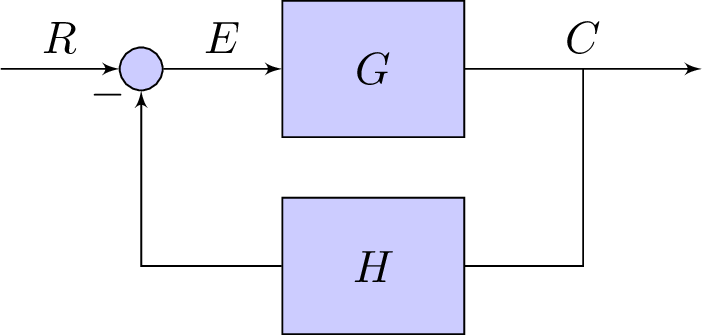
\includegraphics[width=0.7\linewidth]{images/ELEC460Notes-figure0.png}
	\caption{Block Diagram}
	\label{fig:elec460notes-figure0}
\end{figure}

\else
\begin{figure}[h]
	\centering
	\tikzstyle{block} = [draw, fill=blue!20, rectangle, minimum height=3em, minimum width=4em]
	\tikzstyle{block2} = [draw, fill=blue!20, rectangle, minimum height=2em, minimum width=2em]
	\tikzstyle{sum} = [draw, fill=blue!20, circle, node distance=1cm]
	\tikzstyle{input} = [coordinate]
	\tikzstyle{output} = [coordinate]
	\begin{tikzpicture}[auto, >=latex']
	% Nodes
	\node [input] (input) {};
	\node [sum, right = 1cm of input] (sum) {};
	%\node [block2, right = 1cm of sum] (system) {$K$};
	\node [block, right = 1cm of sum] (system2) {$G$};
	\node [output, right = 2cm of system2] (output) {};
	\node [block, below = 0.5cm of system2] (h) {$H$};
	% Arrows
	\draw [draw,->] (input) -- node {$R$} (sum);
	\draw [->] (sum) -- node {$E$} (system2);
	%\draw [->] (system) -- (system2);
	\draw [->] (system2) -- node (y) {$C$}(output);
	\draw [-] (y) |- (h) {} ;
	\draw [->] (h) -| node[pos=0.99] {$-$}  node [near end] {} (sum);
	\end{tikzpicture}  
	\caption{Error signal: $E=R-C$}
	\label{fig:sse}
\end{figure}
\fi

The steady-state error (if it exists) is defined by
\begin{equation}
	\label{eq:sse}
	e_\sse := \lim_{t\to\infty} e(t).
\end{equation}

If the system is stable, one can apply the Finaly Value Theorem to obtain
\[
\lim_{t\to\infty} e(t) = \lim_{s\to 0} sE(s).
\]

In general, one would like the steady-state error to be as small as
possible, ideally zero.

\subsection{System type and steady-state error}

In general, to calculate the steady-state error, one uses the FVT as
in equation~(\ref{eq:sse}). However, if the system is stable and
\emph{unity-feedback}, then one can determine the system type and use
this information to obtain the steady-state error much more easily.

Let $G$ be the feedforward transfer function. Assume that $G$ is
written as
\[
G=\frac{N(s)}{s^kD(s)},
\]
where $N$ and $D$ are not factorizable by $s$. Then the type of the
system is given by the integer $k$. Fig.~\ref{fig:systype} shows the
general form of systems of types 1, 2 and 3.

\begin{figure}[h]
	\hspace{1.5cm}\textbf{Type 0}\hspace{3cm}\textbf{Type
		1}\hspace{3cm}\textbf{Type 2}\\
	\vspace{0.1cm} 
	
	\centering \tikzstyle{block} = [draw, fill=blue!20,
	rectangle, minimum height=3em, minimum width=3em]
	\tikzstyle{controller} = [draw, fill=red!20, rectangle, minimum
	height=3em, minimum width=4em] \tikzstyle{sum} = [draw,
	fill=blue!20, circle, node distance=1cm] \tikzstyle{input} =
	[coordinate] \tikzstyle{output} = [coordinate]
	\begin{tikzpicture}[auto, >=latex']
	% Nodes
	\node [input] (input) {};
	\node [sum, right = 0.5cm of input] (sum) {};
	\node [block, right = 0.5cm of sum] (system) {$\frac{N_0(s)}{D_0(s)}$};
	\node [output, right = 1cm of system] (output) {};
	\node [input, below = 0.5cm of system] (m) {};
	% Arrows
	\draw [draw,->] (input) -- node {$R$} (sum);
	\draw [->] (sum) -- node {} (system);
	\draw [->] (system) -- node (y) {$C$}(output);
	\draw [-] (y) |- (m) {} ;
	\draw [->] (m) -| node[pos=0.99] {$-$}  node [near end] {} (sum);
	\end{tikzpicture}  
	\hspace{0.5cm}
	\begin{tikzpicture}[auto, >=latex']
	% Nodes
	\node [input] (input) {};
	\node [sum, right = 0.5cm of input] (sum) {};
	\node [block, right = 0.5cm of sum] (system) {$\frac{N_1(s)}{sD_1(s)}$};
	\node [output, right = 1cm of system] (output) {};
	\node [input, below = 0.5cm of system] (m) {};
	% Arrows
	\draw [draw,->] (input) -- node {$R$} (sum);
	\draw [->] (sum) -- node {} (system);
	\draw [->] (system) -- node (y) {$C$}(output);
	\draw [-] (y) |- (m) {} ;
	\draw [->] (m) -| node[pos=0.99] {$-$}  node [near end] {} (sum);
	\end{tikzpicture}  
	\hspace{0.5cm}
	\begin{tikzpicture}[auto, >=latex']
	% Nodes
	\node [input] (input) {};
	\node [sum, right = 0.5cm of input] (sum) {};
	\node [block, right = 0.5cm of sum] (system) {$\frac{N_2(s)}{s^2D_2(s)}$};
	\node [output, right = 1cm of system] (output) {};
	\node [input, below = 0.5cm of system] (m) {};
	% Arrows
	\draw [draw,->] (input) -- node {$R$} (sum);
	\draw [->] (sum) -- node {} (system);
	\draw [->] (system) -- node (y) {$C$}(output);
	\draw [-] (y) |- (m) {} ;
	\draw [->] (m) -| node[pos=0.99] {$-$}  node [near end] {} (sum);
	\end{tikzpicture}  
	\caption{Systems of types 0, 1 and 2. Note that $N_0, N_1, N_2, D_0,
		D_1, D_2$ should not be factorizable by $s$.}
	\label{fig:systype}
\end{figure}

Let us carry further the computation of the steady-state error for a
stable unity-feedback system.
\[
sE(s) = s(R(s)-C(s)) = s\left(R(s)-\frac{G(s)}{1+G(s)}R(s)\right)=\frac{s}{1+G(s)}R(s).
\]

For unit-step input, one has $R(s)=1/s$. Thus,
\[
sE(s) = \frac{s}{1+G(s)}*\frac{1}{s} = \frac{1}{1+G(s)}
\xrightarrow[s\to 0]{}\frac{1}{1+\lim_{s\to 0}G(s)}.
\]
For a system of type 0, one has
\[
\lim_{s\to 0}G(s) = \lim_{s\to 0}\frac{N_0(s)}{D_0(s)} = \frac{N_0(0)}{D_0(0)}.
\]
Thus, the steady-state error of a system of type 0 for unit-step input
is given by
\[
e_\sse = \frac{1}{1+\frac{N_0(0)}{D_0(0)}}.
\]

Carrying out similar calculations, one obtains the following table,
which shows the steady-state errors of systems of types 0, 1, 2, 3 for
unit-step, unit-ramp and unit-parabola inputs.

\begin{table}[htp]
	\centering
	\begin{tabular}{|c|c|c|c|}
		\hline
		System type&Step input&Ramp input&Parabolic input\\\hline
		Type 0&$\frac{1}{1+K_p}$&$\infty$&$\infty$\\\hline
		Type 1&0&$\frac{1}{K_v}$&$\infty$\\\hline
		Type 2&0&0&$\frac{1}{K_a}$\\\hline
		Type 3&0&0&0\\\hline
	\end{tabular}
	\caption{Steady-state errors of systems of different types and for
		different inputs.}
	\label{tab:systype}
\end{table}

The constants $K_p$, $K_v$, and $K_a$ are defined as below
\begin{itemize}
	\item for a system of type 0, $K_p:=\frac{N_0(0)}{D_0(0)}$ (position constant);
	\item for a system of type 1, $K_v:=\frac{N_1(0)}{D_1(0)}$ (velocity constant);
	\item for a system of type 2, $K_a:=\frac{N_2(0)}{D_2(0)}$
	(acceleration constant).
\end{itemize}

\subsection{Other Block Diagrams}
In the Laplace domain, we have
\[
I = K_D(sZ_\re-sZ) + K_P(Z_\re-Z) = (K_Ds+K_P)(Z_\re-Z),
\]
which leads to the following block diagram.

\begin{figure}[H]
	\label{fig:examplesystempd}
	\centering
	\tikzstyle{block} = [draw, fill=blue!20, rectangle, minimum height=3em, minimum width=4em]
	\tikzstyle{controller} = [draw, fill=red!20, rectangle, minimum height=3em, minimum width=4em]
	\tikzstyle{sum} = [draw, fill=blue!20, circle, node distance=1cm]
	\tikzstyle{input} = [coordinate]
	\tikzstyle{output} = [coordinate]
	\begin{tikzpicture}[auto, >=latex']
	% Nodes
	\node [input] (input) {};
	\node [sum, right = 1cm of input] (sum) {};
	\node [controller, right = 1cm of sum] (system) {$K_D s + K_P$};
	\node [block, right = 1cm of system] (system2) {$\frac{k}{ms^2}$};
	\node [output, right = 2cm of system2] (output) {};
	\node [input, below = 0.5cm of system] (m) {};
	% Arrows
	\draw [draw,->] (input) -- node {$Z_\re$} (sum);
	\draw [->] (sum) -- node {} (system);
	\draw [->] (system) -- node {$I$} (system2);
	\draw [->] (system2) -- node (y) {$Z$}(output);
	\draw [-] (y) |- (m) {} ;
	\draw [->] (m) -| node[pos=0.99] {$-$}  node [near end] {} (sum);
	\end{tikzpicture}  
	\caption{Proportional-derivative control.}
\end{figure}

\begin{figure}[H]
	\label{fig:lag}
	\centering
	\tikzstyle{block} = [draw, fill=blue!20, rectangle, minimum height=3em, minimum width=4em]
	\tikzstyle{controller} = [draw, fill=red!20, rectangle, minimum height=3em, minimum width=4em]
	\tikzstyle{sum} = [draw, fill=blue!20, circle, node distance=1cm]
	\tikzstyle{input} = [coordinate]
	\tikzstyle{output} = [coordinate]
	\begin{tikzpicture}[auto, >=latex']
	% Nodes
	\node [input] (input) {};
	\node [sum, right = 1cm of input] (sum) {};
	\node [controller, right = 1cm of sum] (con1) {$\frac{s+p_c}{s+z_c}$};
	\node [controller, right = 1cm of con1] (con2) {$K_D s + K_P$};
	\node [block, right = 1cm of con2] (system2) {$\frac{k}{ms^2}$};
	\node [output, right = 2cm of system2] (output) {};
	\node [input, below = 0.5cm of con2] (m) {};
	% Arrows
	\draw [draw,->] (input) -- node {$Z_\re$} (sum);
	\draw [->] (sum) -- (con1);
	\draw [->] (con1) -- (con2);
	\draw [->] (con2) -- node {$I$} (system2);
	\draw [->] (system2) -- node (y) {$Z$}(output);
	\draw [-] (y) |- (m) {} ;
	\draw [->] (m) -| node[pos=0.99] {$-$}  node [near end] {} (sum);
	\end{tikzpicture}  
	\caption{Lag compensation in series with PD control.}
\end{figure}

\begin{figure}[H]
	\label{fig:integral}
	\centering
	\tikzstyle{block} = [draw, fill=blue!20, rectangle, minimum height=3em, minimum width=4em]
	\tikzstyle{controller} = [draw, fill=red!20, rectangle, minimum height=3em, minimum width=4em]
	\tikzstyle{sum} = [draw, fill=blue!20, circle, node distance=1cm]
	\tikzstyle{input} = [coordinate]
	\tikzstyle{output} = [coordinate]
	\begin{tikzpicture}[auto, >=latex']
	% Nodes
	\node [input] (input) {};
	\node [sum, right = 1cm of input] (sum) {};
	\node [controller, right = 1cm of sum] (system) {$\frac{K}{s}$};
	\node [block, right = 1cm of system] (system2) {$\frac{1}{Ts+1}$};
	\node [output, right = 2cm of system2] (output) {};
	\node [input, below = 0.5cm of system] (m) {};
	% Arrows
	\draw [draw,->] (input) -- node {$R$} (sum);
	\draw [->] (sum) -- node {} (system);
	\draw [->] (system) --  (system2);
	\draw [->] (system2) -- node (y) {$C$}(output);
	\draw [-] (y) |- (m) {} ;
	\draw [->] (m) -| node[pos=0.99] {$-$}  node [near end] {} (sum);
	\end{tikzpicture}  
	\caption{First order system with integral controller.}
\end{figure}

\begin{theorem}{Anime}
	A set $\mathcal{D}(G)$ in dense in $L^2(G)$, $|\cdot|_0$. 
\end{theorem}

%------------------------------------------------

\section{Definitions}\index{Definitions}

This is an example of a definition. A definition could be mathematical or it could define a concept.

\begin{definition}{Cute}{label4}
	Given a vector space $E$, a norm on $E$ is an application, denoted $||\cdot||$, $E$ in $\mathbb{R}^+=[0,+\infty[$ such that:
	\begin{align}
	& ||\mathbf{x}||=0\ \Rightarrow\ \mathbf{x}=\mathbf{0}\\
	& ||\lambda \mathbf{x}||=|\lambda|\cdot ||\mathbf{x}||\\
	& ||\mathbf{x}+\mathbf{y}||\leq ||\mathbf{x}||+||\mathbf{y}||
	\end{align}
\end{definition}

%------------------------------------------------

\section{Notations}\index{Notations}

\begin{example}{Real Cute}{label5}
	Given an open subset $G$ of $\mathbb{R}^n$, the set of functions $\varphi$ are:
	\begin{enumerate}
		\item Bounded support $G$;
		\item Infinitely differentiable;
	\end{enumerate}
	a vector space is denoted by $\mathcal{D}(G)$. 
\end{example}

%------------------------------------------------

\section{Remarks}\index{Remarks}

This is an example of a remark.

\begin{remark}
	The concepts presented here are now in conventional employment in mathematics. Vector spaces are taken over the field $\mathbb{K}=\mathbb{R}$, however, established properties are easily extended to $\mathbb{K}=\mathbb{C}$.
\end{remark}

%------------------------------------------------

\section{Corollaries}\index{Corollaries}

This is an example of a corollary.

\begin{corollary}{definition}{label}
	The concepts presented here are now in conventional employment in mathematics. Vector spaces are taken over the field $\mathbb{K}=\mathbb{R}$, however, established properties are easily extended to $\mathbb{K}=\mathbb{C}$.
\end{corollary}

\nocite{*}

\chapter{References}
\printbibliography[heading=none]
\end{document}